\chapter{Überwachtest Lernen}
\label{sec:learning}

\emph{Überwachtes Lernen} ist ein Wissenschaftsgebiet des \emph{Maschinellen Lernen}. Es existieren verschiedene Definitionen für Maschinelles Lernen. Eine der meist zitierten Definitionen lauteet wie folgt:

\begin{quote}
	A Computer Program is said to learn from experience $E$ with respect to some class of tasks $T$ and performance measure $P$, if its performance at tasks in $T$, as measured by $P$, improves with experience $E$.\cite[S. 2]{machine_mitchell}
\end{quote}

Diese weitreichende Definition lässt sich auf verschiedene Wissenschaftsgebiete anwenden. Ein Beispiel ist ein Computer Programm, welches lernt, Dame zu spielen. Angewandt auf die eben genannte Definition lassen folgende Aufgabenbereiche definieren:

\begin{itemize}
\item \textbf{Task} $T$: Dame spielen.
\item \textbf{Performance Measure} $P$: Prozentsatz gewonnener Spiele gegen Gegner
\item \textbf{Training Experience} $E$: Übungsspiele gegen sich selber.
\end{itemize}

Selbstverständlich könnten $P$ und $E$ in diesem Beispiel beliebig anders gewählt werden. $P$ könnte auch die Freude sein, die der menschliche Gegenspieler beim Spiel erfindet. \cite[S. 2 -3 ]{machine_mitchell}

Die Klasse an Aufgaben, die für diese Arbeit Bedeutung besitzen, ist die des \emph{Überwachten Lernens}. Beim Überwachten exisitert ein \emph{Trainings-Datensatz} mit korrekten Antworten auf die Problem-Fragestellung. Der Algorithmus generalisiert diese Trainings-Beispiele, um auf alle möglichen Datensätze die richtige Lösung zu gewährleisten. \cite[S 6]{machine_marsland}

Ein Beispiel für ein Problem des überwachten Lernens ist die \emph{Erkennung von Handschrift}. Die Aufgabenbereiche werden folgendermaßen identifiziert: 

\begin{itemize}
	\item \textbf{Task} $T$: Erkennung handgeschriebener Worte in Bildern und Zuordnung zu dem tatsächlichen Wort. 
	\item \textbf{Performance Measure} $P$: Prozentsatz korrekt erkannter Wörter
	\item \textbf{Training experience} $E$: Eine Datenbank mit handgeschriebener Wörter und mit dem tatsächlich geschriebenen Wort. \cite[S. 3 - 4]{machine_mitchell}
\end{itemize}

Dieses Problem gehört zur Unterkategorie der \emph{Klassifzierung}, beschrieben in Kapitel \ref{sec:classification}. 

Eine zweite Klasse an Aufgaben des überwachten Lernens, die  Bedeutung in dieser Arbeit hat, ist die \emph{Regression}. Ein Beispiel für eine Regressionsaufgabe ist die \emph{Schätzung des Verkaufspreieses einges gebrauchten PKWs}. Folgende Aufgebenbereiche werden identifiziert:

\begin{itemize}
	\item \textbf{Task} $T$: Schätzung des Marktwertes eines gebrauchten PKWs. 
	\item \textbf{Performance Measure} $P$: Abweichung des geschätzten Wertes zum tatsächlichen Verkaufswert
	\item \textbf{Training experience} $E$: Eine Datenbank mit gebrauchten PKWs und ihrem tatsächlichen Verkaufswert.
\end{itemize}

\section{Klassifizierung}
\label{sec:classification}

Das Klassifzierungs-Problem wird folgendermaßen modelliert: 

Es existieren \emph{Instanzen} $x$. Jede Instanzen hat eine Reihe an Eigenschaften, bezeichnet als \emph{Features} oder \emph{Attribute} $f$, wobei jedes Feature einen eigenen Wertebereich, bezeichnet als \emph{Domain} hat. Menge aller möglichen Feautre-Kombinationen wird als \emph{Feature-Raum} $X$ bezeichnet.  

\begin{equation}
\label{eq:feature-space}
\begin{gathered}
\text{Feature-Raum :} \qquad X = \{\  dom(f_1) \times , \ldots, \times dom(f_n)\ \} \\
\text{Instanz :} \qquad  x \in X 
\end{gathered}
\end{equation}

Außerdem exisistiert eine Menge an \emph{Klassen} $C = \{1, \ldots , k\}$. Die \emph{Klassifizierungs-Funktion}, \emph{Predictor}  oder \emph{Classifier} $c$ bestimmt für eine Instanz eine Klasse.

\begin{equation}
\label{eq:classifier-classes}
\begin{gathered}
\text{Classes :} \qquad C = \{ 1 , \ldots , k \} \\
\text{Classifier: } \qquad  c: X \mapsto C
\end{gathered}
\end{equation}

Es gibt einen Datensatz $D$ mit einer Menge an Instanzen. Für jede der Instanzen ist die zugehörige Klasse bekannt. Ein Paar aus Instanz und Klasse wird als \emph{Example} $e$ bezeichnet. Die einer Instanz $x_i$ zugewiesenen Klasse $c_i$ wird als \emph{Label} beschrieben.
 
\begin{equation}
\label{eq:dataAndExample}
\begin{gathered}
\text{Datensatz :} \qquad D = \{ \langle x_1, c_1 \rangle, \ldots , \langle x_n, c_n \rangle  \} \\
\text{Example: } \qquad  e \in D
\end{gathered}
\end{equation}

Die Fehlerfunktion $E$ zählt für einen Datensatz die Menge aller nicht richtig klassifzierten Instanzen

\begin{equation}
\text{E}(D,c) = \counti_{\langle x_i, c_i \rangle \in D} (c(x_i) \neq c_i)
\end{equation}

Das Ziel des Klassfikations-Problems ist es, diejenige Funktion $C$ zu finden, die für einen Test-Datensatz $D_{test} \subseteq D$ die Anzahl falsch klassifzierter Examples minimiert. Nach dem in Kapitel \ref{sec:learning} vorgestellten Muster nach $T$, $P$ und $E$ ergibt sich folgende Aufgabenbeschreibung. \cite[S. 8 - 9]{learning_cart_dobra} \cite[S. 14]{cart_loh} \cite[S. 7 - 10, 18]{machine_marsland}

\begin{itemize}
	\item \textbf{Task} $T$: Für einen Test-Datensatz $D_{test} \subseteq D$, finde eine Klassfikations-Funktion $c$, die die Funktion $E$ minimiert, das heißt: $\quad E(D_{Test}, c) \mapsto min$
	\item \textbf{Performance Measure} $P$: Die Fehler-Funktion $E(D_{test}, c)$.
	\item \textbf{Training experience} $E$: Ein Trainings-Datensatz $D_{training} \subseteq D$ 
\end{itemize}

Im Zusammenahang mit Klassifikation haben die Klassen $C$ die Eigenschaft, dass die Klassen eine \emph{qualitativen} Charakter, und keinen \emph{quantitativen}. Das heißt, dass die Klassen untereinander keine hierarchische Ordnung besitzen, bei der eine Klasse \glqq besser ist als die andere\grqq{}. Außerdem handelt es sich um eine diskrete Menge, und keinen kontinuierlichen Zahlenbereich. \cite[S. 127]{statistical_learning}. Ein besonderer Fall der Klassifikation ist ein sogenannter \emph{binärer Klassfikator}, bei dem es nur zwei Klassen gibt: $C = \{0, 1\}$ (oder $C = \{yes, no\}$ ). %Citatioooon
Die Domains der Features können ebenfalls qualitativer natur sein, das heißt einen Wert in einem diskreten, ungeordneten Raum annehmen, oder  quantitativer Natur, das heißt, einen Wert in einem kontinuierlichen, geordneten Zahlenraum annehmen. \cite[S. 54]{machine_mitchell}

Eine andere Art und Weise, die Aufgabenstellung der Klassifikation zu betrachten, ist die \emph{Generalisation zur Prongnose}. Das heißt, dass die Ableitung der Klassen aus den Instanzen des Datensatzes verallgemeinert wird, um in Zukunft für neue, noch nicht bekannte Instanzen die Klasse vorhersagen (prognostizieren) zu können. \cite[S. 6 - 7]{machine_marsland}

Tabelle \ref{tab:classfication_example} gibt einen Beispiel-Datensatz für eine Klassifkationsproblem. In diesem Beispiel geht es darum, ob abhängig von der Tageszeit und der Temperatur ein Federball-Match Spaß gemacht hat, oder nicht. Das Problem wird folgendermaßen modelliert:

\begin{itemize}
\item Es gibt zwei Features: $f_1 = Temperatur$, mit $dom(f_1) = R$, ein quantitives Feature. $f_2 = Tageszeit$, mit $dom(f_2) = {morgens, mittags, abends}$, ein qualitatives Feature. Der Feature-Raum ist $X = {dom(f_1) \times dom(f_2) }$.
\item Es gibt zwei Klassen, $C = {Ja, Nein}$.
\item Der Datensatz hat fünf Instanzen, $D = \{x_1, \ldots, x_5 \}$. Für jede Instanz ist das Label $c_1 , \ldots , c_5$ bekannt, welches besagt, ob das Federball spielen Spaß gemacht hat, oder nicht. 
\end{itemize}

\begin{table}[h]
	\centering
	\caption{Beispieldatensatz D für eine Klassifikation}
	\label{tab:classfication_example}
	\begin{tabular}{cccc}
		\toprule
		$x_i$      & Temperatur & Tageszeit & $c_i$ = Spaß? \\\midrule
		$x_1$  & 20                & morgens          & Ja           \\
		$x_2$  & 15                & abends           & Ja           \\
		$x_3$  & 8                 & mittags          & Nein         \\
		$x_4$  & 23                & mittags          & Ja           \\
		$x_5$  & 10                & morgens          & Nein       \\ \bottomrule 
	\end{tabular}
\end{table}

Das Ziel ist, in Zukunft abschätzen zu können, allein durch die Kenntniss der Temperatur und Tageszeit abschätzen zu können, ob das Federball-Spielen Spaß machen wird, damit man von vorneherein keine Matches beginnt, die keine Aussicht auf Spaß haben. An dieser Stelle wählt man einen Algorithmus, der einen Classifier baut, der dieses Problem löst. 

Es gibt eine Reihe an Algorithmen, die Classifikatoren nach unterschiedlichen Methoden erstellen. Beispiele sind für \emph{k-NN}, \emph{Support-Vector-Maschienen} oder \emph{künstliche Neuronale Netze}. Eine Klasse an Klassifikations-Algorithmen, die in dieser Arbeit Anwendung finden, sind die sogenannten \emph{Entscheidungsbäume}

\subsection{ID3}
\label{sec:id3}

Es gibt drei Algorithmen zur Erzeugung von Entscheidungsbäumen, die weitreichende Einsatz finden: \emph{ID3}, \emph{C.45} und \emph{CART}, wobei die letzteren Erweiterungen der grundlegenden Idee des \emph{ID3}-Algorithmus darstellen. Daher wird an dieser Stelle zuerst der \emph{ID3}-Algorithmus vorgestellt. 

Es wird zunächst davon ausgegangen, dass alle Features diskret und nicht kontinuierlich sind. Tabelle \ref{tab:id3_example} gibt einen Beispieldatensatz, an dessen Beispiel ein Classificator mit Hilfe des ID3 erzeugt wird. Es geht ähnlich dem Beispiel aus Tabelle \ref{sec:classification} um die Frage, ob Federball-Spielen abhängig von Temperatur und Tageszeit Spaß macht, nur sind in diesem Fall alle Features diskret. 

\begin{table}[h]
	\centering
	\caption{Beispieldatensatz D für die Kassfikation mit ID3}
	\label{tab:id3_example}
	\begin{tabular}{cccc}
		\toprule
		$x_i$    &Temperatur   & Tageszeit & $c_i$ = Spaß? \\\midrule
		$x_1$  & warm                & Tag          & Ja           \\
		$x_2$  & kalt                & Tag          & Ja           \\
		$x_3$  & normal                & Nacht          & Nein         \\
		$x_4$  & kalt                & Nacht          & Nein           \\
		$x_5$  & normal                & Tag         & Ja       \\
		$x_6$  & warm                & Nacht          & Ja       \\ \bottomrule  
	\end{tabular}
\end{table}

Abbildung \ref{img:id3tree} zeigt einen Klassifikator, den der ID-3 Algorithmus für diesen Datensatz baut. Es handelt sich um einen Entscheidungsbaum. In Jedem Knoten steht ein Feature, welches einen Ast für jeden möglichen Wert dieses Features bildet. In den Blättern stehen die Klassen.\cite[S. 134]{machine_marsland}

\begin{figure}[h]
	\centering
	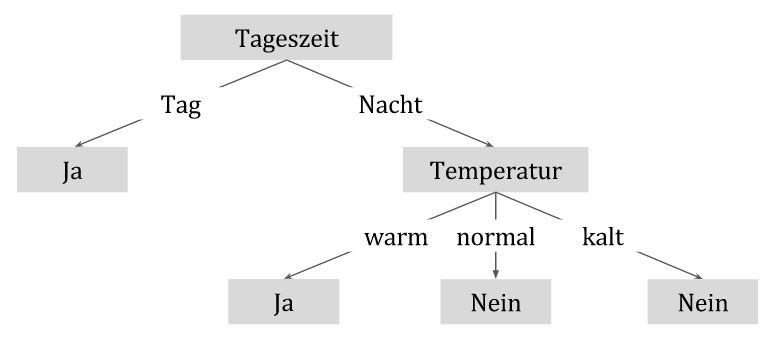
\includegraphics[width=0.6\textwidth]{bilder/id3tree.png}
	\caption{Entscheidungsbaum, der durch den ID3-Algorithmus für den Datensatz aus Beispiel \ref{tab:id3_example} erzeugt wurde.}
	\label{img:id3tree}
\end{figure}

Der Entscheidungsbaum lässt sich in eine Reihe von \texttt{if ... then ...}
-Regeln transformieren. Jeder Weg von der Wurzel bis zu einem Blatt ergibt eine Entscheidungsregel, bei der Feauture-Werte der betretenen Kanten konjunktiv Verknüpft werden und die Klasse implizieren. Die Entscheidungsregeln für den Baum aus Abbildung 	\ref{img:id3tree} sind: \cite[S. 134]{machine_marsland}

\begin{itemize}
\item \texttt{if}  \emph{Tageszeit = Tag} \texttt{then} \emph{Spaß = Ja}
\item \texttt{if}  \emph{Tageszeit = Nacht} \texttt{and} \emph{Temperatur = warm} \texttt{then} \emph{Spaß = Ja}
\item \texttt{if}  \emph{Tageszeit = Nacht} \texttt{and} \emph{Temperatur = normal} \texttt{then} \emph{Spaß = Nein}
\item \texttt{if}  \emph{Tageszeit = Nacht} \texttt{and} \emph{Temperatur = kalt} \texttt{then} \emph{Spaß = Nein}
\end{itemize}

Der Klassifikator, das heißt der Entscheidungsbaum,  wird beim ID3 Algorithmus nach folgenden Muster erstellt:
Der Baum wird Top-Down erzeugt, dass heisst beginnend bei der Wurzel bis zu den Blättern. Da in jedem Knoten genau ein Feature  aufgespalten wird, wird an der Wurzel die Frage gestellt \glqq \emph{Welches Feature sollte zuerst getestet werden?}\grqq . Um diese Frage zu beantworten, wird jedes Feature einem statistischen Test unterzogen und festzustellen, wie \glqq gut\grqq{} es zur Klassifikation der Trainings-Daten beiträgt. Das \glqq beste\grqq{} Attribut wird ausgewählt und als Wurzel festgelegt. Nun wird ein Kind für jeden möglichen Wert des Features gebildet. Der Datensatz des Elternknotens wird in disjunkte Teilmengen aufteilt, wobei jedes Kind die Untermenge erhält, die den jeweiligen Feature-Wert bestitzt. Daraufhin beginnt für jedes Kind der Prozess des Auswählen des \glqq besten\grqq{} Attributes von vorn. Ein Kind wird dann zu einem Blatt, wenn seine Teilmenge an Daten nur noch aus Instanzen einer Klasse besteht und somit kein weiteres Aufteilen notwendig ist.\cite[S. 55]{machine_mitchell}

Das Wort \glqq gut\grqq{} wurd ein dieser Beschreibung in Anführungsstrichen geschrieben, da es subjektiv ist und quantifiziert werden muss. Zur Quantifizierung der Information wird die Entropie nach Formel \ref{eq:entropy} als Hilfsmittel definiert. $p_i$ ist die Wahrscheinlichkeit, dass in einem Datensatz $D$ eine Instanz mit der Klasse $i \in C$ angetroffen wird.

\begin{equation}
H(p) = -\sum_{i \in C} p_i \cdot \log_{2} p_i
\label{eq:entropy}
\end{equation}

Die Entropie quantifiziert die \emph{Unreinheit des Datensatzes}. Angenommen, ein Datensatz hat zwei Klassen, $C = \{+,-\}$. Existiert der gesamte Datensatz nur aus einer der beiden Klasse, ist die Entropie $- p_{+} \log_{2} p_{+}- p_{-}  \log_{2} p_{-} = -1 log_{2} 1 -0 log_{2} 0 = 0$. Das heißt, dass die \emph{Unreinheit des Datensatzes} $0$  beträgt. Ist die \emph{Unreinheit des Datensatzes} hingegen maximal, das heißt es liegen exakt 50\% positive und 50\% negative Samples vor, ist die Entropie $- p_{+} \log_{2} p_{+} - p_{-}  \log_{2} p_{-} = -0.5 log_{0.5} 1 - 0.5 log_{2} 0.5 = 1$. \cite[S. 135]{machine_marsland}

Es ist das Attribut in einem Knoten zu wählen, welches den höchsten \emph{Informatoinsgewinn} gewährleistet, das heißt, zu einer bestmöglichen \emph{Reinheit} bei der alleinigen Unterteilung des Datensatzes auf Basis dieses Attributs führt. Der informationsgewinn eines Features $f$ für den Datensatz $D$ wird nach Formel \ref{eq:informationGain} definiert. $v$ sind alle möglichen Werte dieses Features. $|D|$ beschreibt die Anzahl an Instanzen des Datensatzes. $D_v$ ist die Untermenge an Instanzen, die für das Feature $f$ den Wert $v$ besitzen.\cite[S. 136 - 137]{machine_marsland}

\begin{equation}
\text{Gain}(D,f) = H(D) - \sum_{v \in dom(f)} \frac{|D_v|}{|D|} H(D_v)
\label{eq:informationGain}
\end{equation}

Für das Beispiel aus Tabelle \ref{img:id3tree} ergibt sich für den ersten Test folgende Berechnung des Informationsgewinnes der beiden Features \emph{Temperatur} und \emph{Tageszeit}. Da die Tageszeit den höheren Informationsgewinn gewährleistet, wird dieses Features in der Wurzel gewählt. 

\begin{equation}
H(D) = - p_{+} \log_{2} p_{+} - p_{-}  \log_{2} p_{-} = -\frac{4}{6} \log_{2} (\frac{4}{6}) -\frac{2}{6} \log_{2}( \frac{2}{6} ) = 0.91
\end{equation}
\begin{equation}
\begin{split}
Gain(D,Tageszeit) = 0.91 - \Big( \overbrace{\frac{3}{6} \cdot (-\frac{3}{3} \log_{2} \frac{3}{3} -  -\frac{0}{3} \log_{2} \frac{0}{3} }^{Tag}   )\ \quad \quad \quad \; \\
\underbrace{\frac{3}{6} \cdot (-\frac{1}{3} \log_{2} \frac{1}{3} -  -\frac{2}{3} \log_{2} \frac{2}{3} }_{Nacht}   \Big)  = 0.86
\end{split}
\end{equation}

\begin{equation}
\begin{split}
Gain(D,Temperatur) =  0.91 - \Big( \overbrace{\frac{2}{6} \cdot (-\frac{2}{2} \log_{2} \frac{2}{2} -  -\frac{0}{2} \log_{2} \frac{0}{2} }^{warm}   ) \quad \quad \quad \quad \\
\overbrace{\frac{2}{6} \cdot (-\frac{1}{2} \log_{2} \frac{1}{2} -  -\frac{1}{2} \log_{2} \frac{1}{2} }_{normal}   \quad \quad \quad \quad \\
\overbrace{\frac{2}{6} \cdot (-\frac{1}{2} \log_{2} \frac{1}{2} -  -\frac{1}{2} \log_{2} \frac{1}{2} }_{kalt} 
  \Big)  = 0.66
\end{split}
\end{equation}

Algorithmus\ref{alg:id3} zeigt den Ablauf des ID-3 in Pseudocode. $D$ ist die Menge aller Test-Examples, $X$ ist die Menge aller Features, $C$ ist die Menge aller Klassen, $f_{parent}$ das Feature des momentanen Eltern-Knotens und  $v_{parent}$ der Wert des zum momentan konstruierten Knotens eingehenden Kante. \cite[S. 139]{machine_marsland} \cite[S. 56]{machine_mitchell}

%% Verbessern :O
\begin{algorithm}[H]
	\footnotesize
	\caption{ID3-Algorithmus in Pseudocode}
	\label{alg:id3}
	\begin{algorithmic}[1]
		\State $tree = \{ \}$
		\Function{ID3}{$D, X, C, f_{parent}, v_{parent}$ }
		\State \Comment If all Examples have the same label, return a leaf with that Label
		\If{ $\forall e \in D: \exists k \in C : e.c = k$}
			\State $tree = tree \cup \{(f_{parent}, v_{parrent},k)\}$
			\State \Return 
	
		\Else
			\State \Comment If there are no Features left to test, return a leaf with 
			\State \Comment the most common Label  of the Examples remaining in $D$
			\If{ $isEmpty(X)$}
				\State $tree = tree \cup \{(f_{parent}, v_{parrent}, \text{most common Label in D})\}$
				\State \Return 
			\Else
				\State \Comment Choose the feature that maximizes the Information-Gain to be the next node
				\State $f_{best} = \maxi_{f \in X} Gain(D,f)$
				\State \Comment Add a Branch to this node
				\State  $tree = tree \cup \{(f_{parent}, v_{parrent},f_{best})\}$
				\State \Comment Remove the feature from the set of features
				\State $X_{/f} \gets X / f_{dom}$
				\For{$v \in f_{best}$}
							\State \Comment Calculate the new Dataset $D_{/f}$ by removing all instances with the corresponding value
						\State $D_{/f} \gets \forall e \in D : e.f_{best} = v$
						\State \Comment Recursivly call the algorithm
						\State \Call{ID3}{$D_{/f}, X_{/f}, f_{dom}, v$}
				\EndFor
			\EndIf
		\EndIf
		
		\EndFunction
		
	\end{algorithmic}
\end{algorithm}

Der ID3-Algorithmus hat folgende \textbf{Vorteile}:

\begin{description}
\item[Kurze Entscheidungsbäume] Der Klassifizierer versucht, möglichst kurze Entscheidungsbäume zu bauen, indem Features mit hohem Informationsgewinn bevorzugt werden. Dies ist eine Umsetzung von \emph{Ocam's Razor}: \glqq Bevorzuge die kürzeste Hypothese\grqq{}
\item[Verständlichkeit]  Der Klassifikator ist für den Menschen verständlich, da er sich in Regeln übersetzen lässt (im Gegensatz zu zum Beispiel Neuronalen Netzen). Es existiert die unbewiesene Hypothese, dass der Mensch bei der Klassifizierung intuitiv ähnlich vorgeht wie der ID3-Algorithmus.\cite[S. 63 - 65]{machine_mitchell}
\end{description}

Der ID3-Algorithmus hat folgende \textbf{Nachteile}
\begin{description}
	\item[Nur Diskrete Werte] Der Algorithmus akzeptiert keine kontinuierlichen Werte \cite[S. 72]{machine_mitchell}
	\item[Overfitting] Der Algorithmus neigt zu \emph{Overfitting}. Overfitting bedeutet, dass der erzeugte Klassfikator $c$ zwar einen möglichst geringen Fehler in Bezug auf den \emph{Trainings-Datensatz} hat, es jedoch einen anderen Klassifikator $c'$ gibt, welcher in Bezug auf den Trainings-Datensatz einen höheren Fehler erzeugt, jedoch einen geringeren Fehler als $c$ in Bezug auf \emph{alle möglichen Instanzen dieses Typs} erzeugt. Anders formuliert bedeutet Overfitting, dass der Klassifikator den Trainings-Datensatz \glqq auswendig gelernt hat\grqq{} und nicht mehr genügend generalisiert, um auf im Training nicht enthaltene Instanzen angewandt werden zu können. Overfitting im Zusammenhang mit dem ID-3 Algorithmus wird durch \emph{Rauschen im Trainings-Datensatz} bedingt. Es gibt keinen festen Beweis für das vorhandensein von Overfitting. Methoden zum Feststellen von Overfitting sind:
	\begin{itemize}
		\item Verwendung eines seperaten Test-Datensatzes, welcher bestätigt, dass der für den Trainings-Datensatz erzeugte Klassifikationsfehler auch bei bisher unbekannten Instanzen erzeugt wird.
		\item Verwendung von Statistischen Tests, die eine signifikante Reduktion des Klassifikationsfehlers bei Erweiterung des Entscheidungsbaumes beweisen.
		\item Expertenwissen über applikationstypischen Tiefen von Entscheidungsbäumen.\cite[S. 66 - 70]{machine_mitchell}
	\end{itemize}
	\item[Lokale Maxima] Der Algorithmus bevorzugt greedy Attribute, die zum Zeitpunkt der Berechnung den höchsten Inforamtionsgewinn gewährleisten. Dabei besteht die Gefahr, dass der Algorithmus in ein lokales Maximum läuft.\cite[S. 66 - 70]{machine_mitchell}
\end{description}

\subsection{C4.5}

Der \emph{C4.5}-Algorithmus erweitert den \emph{ID3}, um dessen Nachteile auszumerzen, das heißt die Möglichkeit der Einführung kontinuierlicher Attribute sowie Lösungsansätze für das Overfitting. An dieser Stelle wird der \emph{C4.5} nicht im Detail vorgestellt, sondern die Erweiterungskonzepte vorgestellt. \cite[S. 66]{machine_mitchell}

\subsubsection*{Kontinuierliche Werte}
Der \emph{C4.5} ermöglicht sowohl diskrete als auch kontinuierliche Attribute. Für ein kontinuierliches Attribut wird in ein \emph{boolsches Attribut} entworfen, das heißt ein Attribut mit dem Wertebereich $\{0,1\}$. Zur Abbildung des kontinuierlichen Attributs auf das boolsche Attribut wird durch einen Grenzwert $c$ auf dessen kontinuierlichen Wertebereich festgelegt, in Form von \texttt{if} $f_c > c$ \texttt{then} $1$ \texttt{else} $0$. Abbildung \ref{img:c45_contvalue} visualisiert einen solchen Knoten in einem Entscheidungsbaum. \cite[S. 72]{machine_mitchell}

\begin{figure}[h]
	\centering
	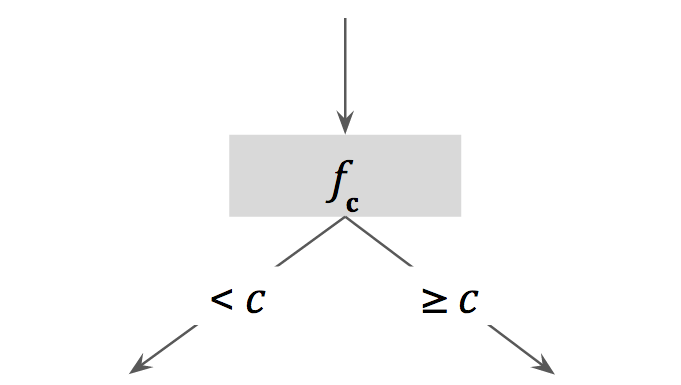
\includegraphics[width=0.3\textwidth]{bilder/c45_contvalue.png}
	\caption{Knoten eines Entscheidungsbaums für kontinuierliche Werte}
	\label{img:c45_contvalue}
\end{figure}

Angenommen, das Attribut \emph{Temperatur} aus Tabelle \ref{tab:id3_example} wird in ein kontinuierliches Attribut umgewandelt, in dem die Temperatur in Grad ausgedrückt wird, wie Tabelle \ref{tab:c45-example} zeigt. 

\begin{table}[h]
	\centering
	\caption{kontinuierliche Attribut-Werte des Features \glqq Temperatur\grqq }
	\label{tab:c45-example}
	\begin{tabular}{lllllll}
		\toprule
		Temperatur & 23   & 5   & 15 & -2 & 18 & 26  \\
		Spaß       & Ja & Ja & Nein & Nein & Ja &Ja \\ \bottomrule
	\end{tabular}
\end{table}

Das Ziel ist nun, denjenigen Grenzwert $c$ zu finden, der den größt möglichen Informationsgewinn für dieses Attribut erzeugt. Das Vorgehen zum finden dieses Grenzwertes ist wie folgt:
\begin{enumerate}
\item Ordnen aller Examples nach dem kontinuerlichen Feature $f_c$. 
\item Identifizierung benachbarter Examples mit unterschiedlicher Klasse als Kandidaten für einen Grenzert
\item Errechnung des Informationsgewinn bei Setzung des Grenzwertes auf den Attributwert jedes gefundenen Kandidaten. Wahl desjenigen Grenzwetes, der den höchsten Informationsgewinn bringt. \cite[S. 73]{machine_mitchell}
\end{enumerate}

%To do: durchrechnen, ob wirklich 15!
Tabelle \ref{tab:c45-example-ordered} zeigt die nach dem Temperatur-Wert geordneten Examples aus Tabelle \ref{tab:c45-example} zur Verdeutlichung des Vorgehens. In diesem Beispiel bilden die Examples mit Temperatur-Werten von $-2, 5, 15$ und $18$ Kandidaten. Der höchste Inforamtionsgewinn wird mit einem Informationsgewinn nach der Entscheidungsregeln \texttt{if} $Temperatur > 15$ \texttt{then} $1$ \texttt{else} $0$.

\begin{table}[h]
	\centering
	\caption{kontinuierliche Attribut-Werte des Features \glqq Temperatur\grqq }
	\label{tab:c45-example-ordered}
	\begin{tabular}{lllllll}
		\toprule
		Temperatur & -2   & 5   & 15     & 18    & 23 & 26  \\
		Spaß            & Nein& Ja  & Nein & Ja & Ja   &Ja \\ \bottomrule
	\end{tabular}
\end{table}

\subsubsection*{Pruning}

Das in Kapitel \ref{sec:id3} als Overfitting beschriebene Problem lässt sich vermeiden, in dem die Tiefe des Entscheidungsbaumes reduziert wird. Diese Begrenzung wird als \emph{Beschneiden} oder \emph{Pruning} bezeichnet. Es gibt grundlegend zwei verschiedene Ansätze: (1) Ab der Überschreitung einer bestimmten Tiefe der Algorithmus frühzeitig stoppen, oder (alias \emph{Pre-Pruning}) (2) zuerst den kompletten Entscheidungsbaum aufbauen und Overfitting zulassen, um diesen im Nachhinein in seiner Tiefe reduzieren (alias \emph{Post-Pruning}). Post-Pruning hat sich insgesamt als erfolgreicher herausgestellt. \cite[S. 68 - 69]{machine_mitchell} 

Eines der am weitesten verbreiteten Post-Pruning-Algorithmen ist das sogenannte \emph{Reduced Error Pruning}. Dabei wird ein Knoten des Entscheidungsbaumes zu einem Blatt umgewandelt und diesem Blatt das Label zugewiesen, welches in seinem Sub-Baum am häufigsten vorkommt. Daraufhin wird der originale Entscheidungsbaum und sowie der beschnittene Entscheidungsbaum verwendet, um den Test-Datensatz zu klassifizieren. Ist der Klassifizierungsfehler des beschnittenen Baumes nicht schlechter als der des originalen Baumes, wird das Pruning übernommen. Dieses Vorgehen wird für jeden Knoten des Entscheidungsbaumes angewandt.

\subsection{Gütemaße binärer Klassifikatoren}

Ein binärer Klassifikation ist eine, bei dem es nur zwei Klassen gibt, das heißt $|C| = 2$. Applikationsabhängig werden die beiden Klassen als \emph{Positive} und \emph{Negative}, $1$ und $0$ oder \emph{True} und \emph{False} beschrieben. Eine Klassifikation, bei der ein tatsächliches Positive richtig als Positive vorhergesagt wird, spricht man von einem \emph{True Positive} [TP]. Wird hingegen ein tatsächliches Positive fälschlicherweise als Negative vorhergesagt, spricht man von einem \emph{False-Negative} [FN]. Das System wird entsprechend für die Klassifikation tatsächlicher Negatives angewandt und ergibt. \emph{True-Negatives} [TN] und \emph{False-Positives} [FP]. Die \emph{Confusion Matrix} in Abbildung \ref{img:Confusion-Matrix} gibt eine Übersicht über die vier möglichen Klassifikations-Ergebnisse.

\begin{figure}[h]
	\centering
	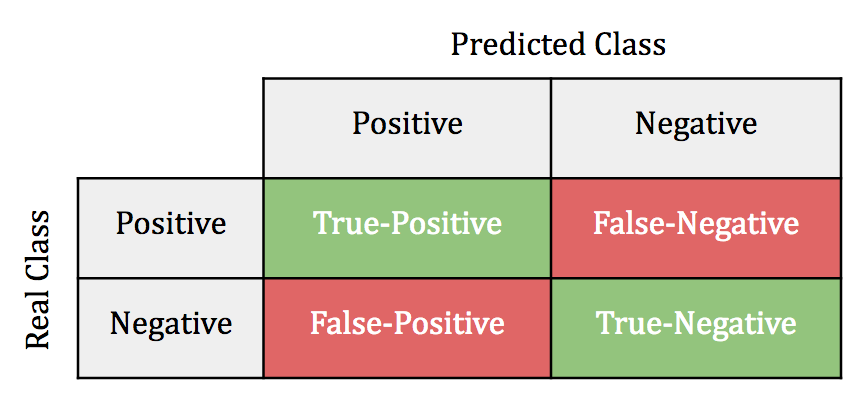
\includegraphics[width=0.4\textwidth]{bilder/Confusion-Matrix02.png}
	\caption{Confusion-Matrix}
	\label{img:Confusion-Matrix}
\end{figure}

Die insgesamte Güte einer Klassifikation wird durch die \emph{Accuracy} nach Formel \ref{eq:accuracy} bestimmt. Eine Accuracy von 100\% bedeutet, dass \emph{alle} Instanzen richtig klassifiziert werden, eine Accuracy von 50\% bedeutet, dass die Hälfte aller Instanzen richtig klassifiziert werden, was der Güte einer rein zufälligen Wahl entspricht.

\begin{equation}
\text{Accuracy} = \frac{TP+TN}{TP+TN+FN+FP}
\label{eq:accuracy}
\end{equation}

Die Accuracy beziffert die insgesamte Performance des Klassifikators, gibt jedoch keinen Aufschluss darüber, ob der Klassifikator eher eine Tendenz zur falschen Klassifizierung von Positives oder Negatives hat. Bei einer Datenbank mit der selben Anzahl an Positives und Negatives kann eine Accuracy von 50\% beispielsweise dadurch entstehen, dass \emph{alle} Instanzen als Positives markiert werden, also sowohl die Positives richtigerweise als Positives, aber die Negatives fälschlicherweise ebenfalls als Positives. Im Umgedrehten Fall ergibt die Klassifizierung aller Instanzen als Negatives ebenfalls eine Accuracy von 50\%. In einem dritten Fall irrt sich die Klassifikator gleich oft bei der Einordnung der Negatives und Positives. Die Maße \emph{Sensitivity} und \emph{Specificity} geben Aufschluss über die Güte der Klassifikation hinsichtlich der Positives und Negatives. Die \emph{Sensitivity}, auch bezeichnet als \emph{True-Positive-Rate}, bemisst den Anteil tatsächlicher Positives, die auch als solche erkannt wurden, nach Formel \ref{eq:sensitivity}. Eine Sensitivity von 100\% bedeutet, dass alle Positives durch den Klassifikator erkannt wurden. Die Erkennungsrate der Negatives hat keinen Einfluss auf die Sensitivity. Eine hohe Sensitivity lässt sich somit \glqq einfach\grqq{} erzielen, in dem man \emph{alle} Instanzen immer als Positives klassifiziert. Die Specificity nach Formel \ref{eq:specificity} bestimmt analog zur Sensitivity den Anteil der korrekt als Negatives bestimmten Instanzen. Ein Klassifikator, der alle Instanzen als Positives markiert, hat zwar eine Sensitivity von 100\%, aber eine Specificity von 0\%. Ergeben zwei verschiedene Klassifikationsmodelle sehr ähnliche Accuracies, hilft die Bestimmung der Sensitivity und Specificity bei der Auswahl des für den Anwendugnsfall Adäquteren Klassifikators. So ist beispielsweise bei der Bestimmung von schweren Krankheiten eventuell ein Klassifikator mit höherer Sensitivity wünschbar, um die Wahrscheinlichkeit zu minimieren, dass die entsprechende Krankheit nicht erkannt wird. \cite{sens-and_spec} \cite{accuracy}

\begin{equation}
\text{Sensitivity} = \frac{TP}{TP+FN}
\label{eq:sensitivity}
\end{equation}

\begin{equation}
\text{Specificity} = \frac{TN}{TN+FP}
\label{eq:specificity}
\end{equation}

\section{Regression}

Während der Klassfikator $c$ bei der Klassifikation die Instanzen auf eine \emph{diskrete, quantitative} Menge abbildet werden, werden bei der Regression die Instanzen auf eine \emph{kontinuierliche, qualitative} Menge abgebildet. Der Klassifikator $c$ wird in der Regression als \emph{Regressor} $r$ bezeichnet, und die Menge, auf die die Instanzen abgebildet werden, als \emph{Output}, \emph{Predicted Attribut} oder \emph{abhängige Variable} $Y$. Wird keine explizite Einschränkung für $Y$ gegeben, so gilt $Y = \mathbb{R}$. \cite[S. 24]{learning_cart_dobra} \cite[S. 8]{machine-marsland}

Die in Kapitel \ref{sec:classification} benannten Definitionen für die Begriffe \emph{Feature-Raum} und \emph{Instanzen} aus Gleichung \ref{eq:feature-space} sowie für \emph{Datensatz} aus Gleichung \ref{eq:dataAndExample} werden bei der Formalisierung der Regression übernommen. Die Defintion von \emph{Classes} und \emph{Classifier} aus Formel \ref{eq:classifier-classes} wird Ersetzt durch \emph{Output} und \emph{Regressor} nach Gleichung \ref{eq:output-regressor}.\cite[S. 24]{learning_cart_dobra}

\begin{equation}
\label{eq:output-regressor}
\begin{gathered}
\text{Output :} \qquad Y = \mathbb{R}\\
\text{Regressor: } \qquad  r: X \mapsto Y
\end{gathered}
\end{equation}

Ein Datensatz $D$ enthält bei der Regression Tupel aus Samples und dem bekannten Output.

\begin{equation}
\text{Datensatz :} \qquad D = \{ \langle x_1, y_1 \rangle, \ldots , \langle x_n, y_n \rangle  \} \\
\end{equation}

Die Fehlerfunktion entspricht dem aus Gleichung \ref{eq:reg-error} als Summe aller quadrieten differenzen zwischen dem tatsächlichen und dem durch den Regressor geschätzten Output definiert.

\begin{equation}
\label{eq:reg-error}
\text{Error :} E(D,r) = \sum_{ \langle x_i, y_i \rangle \in D} ( r(x_i) - y_i )^2
\end{equation}
